%!TEX root = /Users/fort002/Google Drive/Research/Write_ups/Dissertation/Slide-Presentation/Fortin_diss_slides.tex

%%%%% INTRODUCTION %%%%%
\frame
{
\begin{figure}
\begin{center}
\includegraphics[width=\textwidth]{Plots/growth-curves.png}
\caption{ The heights of 10 girls measured at 31 ages.}
\end{center}
\end{figure}
}

\frame
{
\begin{figure}
\begin{center}
\includegraphics[width=3in]{Plots/canadian-weather.pdf}
\caption{ Mean monthly temperatures for Canadian weather stations.}
\end{center}
\end{figure}
}


\frame{
\begin{figure}
        \centering
        \begin{subfigure}[b]{0.44\textwidth}
                \centering
                \includegraphics[width=\textwidth]{Plots/fourier-basis-7.pdf}
                \caption{Fourier basis functions}
        \end{subfigure}
         \begin{subfigure}[b]{0.44\textwidth}
                \centering
                \includegraphics[width=\textwidth]{Plots/bspline-basis-7-order4.pdf}
                \caption{B-spline basis functions}
        \end{subfigure}
 \end{figure}
}

\begin{frame}[t]{}
	\begin{tabular}{c|c|c|}
		& Independent & Dependent \\
		\hline
		Sparse & \includegraphics[width=1.3in]{Plots/canadian-weather.pdf} & \includegraphics[width=1.3in]{Plots/canadian-weather.pdf} \\
		\hline
		Dense & \includegraphics[width=1.3in]{Plots/growth-curves.png} &\includegraphics[width=1.3in]{Plots/canadian-weather.pdf}\\
		\hline
	\end{tabular}
\end{frame}
%--- Next Frame ---%



\frame{
Goals:
\begin{itemize}
\item Represent curves with an empirical basis consisting of functional principal components.
\begin{itemize}
\item FPCs are eigenfunctions that correspond to the covariance function
\item  \structure{$\int_a^bC(s,t)\psi_j(t)dt = \lambda_j\psi_j(t)$}
\end{itemize}
\item Allows spatial structure to be modeled through basis coefficients
\end{itemize}
Outline:
\begin{enumerate}
\item Nonparametric covariance estimation and principal component function estimation
\item Application to phenology data
\item Predicting curves at unobserved locations
\end{enumerate}
}




%%%%% NONPARAMETRIC COVARIANCE FUNCTION ESTIMATION AND EIGENFUNCTION ESTIMATION %%%%%
\frame{
\begin{center}
NONPARAMETRIC COVARIANCE FUNCTION AND PRINCIPAL COMPONENT FUNCTION ESTIMATION FOR FUNCTIONAL DATA
\end{center}
}

\begin{frame}
\frametitle{Smoothing Penalty Approach (univariate case)}
\begin{equation*}
\widehat{f}_{\lambda} = \hspace{.07in}\stackrel[f \in \H]{}{\mbox{arg min}} \left\{ \frac{1}{n}\sum_{i=1}^{n}(y_i - f(x_i))^2 + \lambda\times Pen(f) \right\}.
\label{eq:PLS_norm}
\end{equation*}
\begin{itemize}
\item $Pen(f)$ is a penalty applied to 'non-smooth' functions in order to avoid over fitting the data.
\item $\H$ is an 'appropriate' function space.
\item $\lambda$ is a parameter which governed the trade-off between fitting the data and smoothness of the curve.
\end{itemize}
A reasonable approach is to define $Pen(f) = \int_0^1 (f'')^2dx$. 
\begin{equation*}
\widehat{f}_{\lambda} = \hspace{.07in}\stackrel[f \in \H]{}{\mbox{argmin}} \left\{ \frac{1}{n}\sum_{i=1}^{n}(y_i - f(t_i))^2 + \lambda\ \int_0^1(f'')^2dx \right\}
\label{eq:unpenalized objective function}
\end{equation*}
Okay, so how do we solve for $\hat{f}$?
\end{frame}

%%%%%%%%%%%%%%%%%%
%%%%%%%%%%%%%%%%%
\begin{frame}\frametitle{Spaces generated by positive definite functions}
\begin{itemize}
\item Let $K(x,y)$ be a symmetric positive-definite kernel function. 
\item $\H_K = \{K(\cdot, y), y \in \Real\}$
\end{itemize}
From Mercer's theorem $K(x,y)$ has the representation
\[K(x,y)=\sum_{i=0}^{\infty}\lambda_{i}\phi_{i}(x)\phi_{i}(y)\]
\begin{itemize}
\item $\phi_{i}$ are eigenfunctions of the kernel function $K$
corresponding to eigenvalues $\lambda_{i}$.
\item $\phi_{i}$ are basis for $L_2$.
\end{itemize}
$\H_{K}\subset L_{2}$ contains functions satisfying
\[f(x)=\sum_{i=1}^{\infty}c_{i}\phi_{i}(x)\] 
 for $c_{i} \mbox{ with  }\norm{f}_{\H_K}:= \sum_{i=1}^{\infty}\frac{{c_{i}^{2}}}{\lambda_{i}}<\infty$
\end{frame}

\begin{frame}
The minimization problem becomes
\begin{equation*}
\widehat{f}_{\lambda} = \hspace{.07in}\stackrel[\{c_j\}_{j=1}^{\infty}]{}{\mbox{argmin}} \left\{ \frac{1}{n}\sum_{i=1}^{n}(y_i - \sum_{j=1}^{\infty}c_j\phi_j(x_i))^2 + \lambda\ \sum_{j=1}^{\infty}\frac{c_j^2}{\lambda_j} \right\}
\label{eq:unpenalized objective function}
\end{equation*}
The solution is finite dimensional and has the form
\[
\hat{f}(x)=\sum_{i=1}^{N}b_{i}K(x,x_{i})
\]
This remarkable result is due to the fact that $K(x,y)$ is a 'reproducing' kernel. 

That is great! And it gets better...
\end{frame}
\begin{frame}
The reproducing property: 
\begin{itemize}
\item $f(x_i) = \inner{K(\cdot, x_i)}{f}$
\item $\inner{K(\cdot, x_i)}{K(\cdot, x_j)} = K(x_i, x_j)$
\end{itemize}
implies that for $f(x)=\sum_{i=1}^{N}b_{i}K(x,x_{i})$

\[\left\Vert f\right\Vert _{H_{K}}^{2}=\inner{f}{f}_{H_{K}}=\sum_{i=1}^{N}\sum_{j=1}^{N}b_{i}b_{j}K(x_{i},x_{j})\]

Thus the optimization reduces to minimizing, over choices of vectors $b$, the
following

\[(Y-Kb)'(Y-Kb)+\lambda b'Kb.\]
\end{frame}

\begin{frame}
\frametitle{Side Note: Some (very) useful Hilbert space properties:}

\begin{itemize}
\item tensor sum decomposition: \structure{$\H = \H_0 \tsum \H_1$}
	\begin{itemize}
	\item $f \in \H$ has representation $f = f_0 + f_1$
	\item If $\H_0$, $\H_1$ are RKHS, then \structure{$R = R_0 + R_1$} is r.k. on $\H$.
	\end{itemize}
	\vspace{1cm}
\item tensor product space: If $\H_{<1>}$ and $\H_{<2>}$ are RKHS then
\begin{itemize}
	\item Tensor product space \structure{$\H_{<1>}\tprod \H_{<2>}$} is a RKHS 
	\item $R_{<1>}\tprod R_{<2>}((s_1, t_1), (s_2, t_2)) = \structure{R_{<1>}(s_1, s_2)R_{<2>}(t_1, t_2)}$
	\end{itemize}
\end{itemize}
\end{frame}

\frame{
\frametitle{Back to the original problem...}

 Penelty based on high-order derivative
\begin{equation*}
\widehat{f}_{\lambda} = \hspace{.07in}\stackrel[f \in \H]{}{\mbox{argmin}} \left\{ \frac{1}{n}\sum_{i=1}^{n}(y_i - f(x_i))^2 + \lambda\ \int_0^1(f'')^2dx \right\}
\label{eq:unpenalized objective function}
\end{equation*}

Consider the space $\H =  \{f : f, f' \mbox{ absolutely continuous}, f'' \in L_2[0,1]\}$ with decomposition $\H = \H_0 \tsum \H_1$, where 
  \begin{align*}
  \H_0 &= \left\{f: \int_0^1(f'')^2dx = 0\right\}\\
  \H_1 & = \H \tminus \H_0
  \end{align*}
  The space $\H$ is a RKHS under the inner product
  \begin{align*}
  \inner{f}{g} &= \inner{f}{g}_0 + \inner{f}{g}_1 \\
  			&= \left(\int_0^1fdx\right)\left(\int_0^1gdx\right) + \left(\int_0^1f'dx\right)\left(\int_0^1g'dx\right) + \int_0^1 f''g''dx
  \end{align*}
}
\begin{frame}
\frametitle{¥}
  The minimization problem becomes
  \begin{equation*}
\widehat{f}_{\lambda} = \hspace{.07in}\stackrel[f \in \H]{}{\mbox{arg min}} \left\{ \frac{1}{n}\sum_{i=1}^{n}(y_i - f(x_i))^2 + \lambda\norm{P_1(f)}^2_{\H_1} \right\}.
\end{equation*}
where $P_1(f)=f_1$ is the projection of $f$ onto the space $\H_1$. \\[1cm]
The solution has the form
\begin{equation*}
	\hat{f}(t) = \sum_{j=1}^M d_j\phi_j(t) + \sum_{i=1}^N c_iR_1(x, x_i), 
	\label{eq:unpenalized solution}
\end{equation*}
\end{frame}

\begin{frame}

\begin{table}
\begin{tabular}{|c|c|}
\hline
& Starting from kernel \\[0.3cm]
\hline 
$[0,1]$ &$\hat{f}(t) =  \sum_{i=1}^N c_iR(t, t_i)$ \\[0.3cm]
\hline
$[0,1]\times [0,1]$ & Cai and Yuan (2010) \\[0.3cm]
\hline
\end{tabular}
\end{table}

\begin{table}
\begin{tabular}{|c|c|}
\hline
 & Starting from penalty \\[0.3cm]
\hline 
$[0,1]$ & $\hat{f}(t) = \sum_{j=1}^M d_j\phi_j(t) + \sum_{i=1}^N c_iR_1(t, t_i)$\\[0.3cm]
\hline
$[0,1]\times [0,1]$  & $?$\\[0.3cm]
\hline
\end{tabular}
\end{table}

The focus of our work is to fill in the remaining box, and to derive eigenfunctions for this estimator.
\end{frame}

\begin{frame}\frametitle{Cai and Yuan (2010)}
Assume the sample path of $X$ belongs to an RKHS $H_{K}.$ Then we
can write

\[
X(\cdot)=\sum_{k\geq1}x_{k}\phi_{k}(\cdot)\]


where $x_{k}=(X,\phi_{k})_{L_{2}}$.

The covariance function $C_{0}(s,t)$ is given by

\[
C_{0}(s,t)=\sum_{j,k\geq1}cov(x_{k},x_{j})\phi_{j}(s)\phi_{k}(t)\]


which identifies it with the tensor product space $H(K\otimes K)=H(K)\otimes H(K)$,
an RKHS associated with reproducing kernel

\[
K\otimes K((s_{1},t_{1}),(s_{2},t_{2}))=K(s_{1},s_{2})K(t_{1},t_{2}).\]
\end{frame}

%\begin{frame}
%
%
%For functions $f\in L_{2}([0,1]\times [0,1])$, write
%
%\[
%f(s,t)=\sum_{j,k\geq1}f_{jk}\phi_{j}(s)\phi_{k}(t).\]
%
%
%The product space $H(K\otimes K)$ contains all function $f$ such
%that
%
%\[
%\left\Vert f\right\Vert _{H(K\otimes K)}^{2}\equiv\sum_{j,k\geq1}\frac{{f_{jk}^{2}}}{\lambda_{j}\lambda_{k}}<\infty.\]
%
%\end{frame}

%%%%%%%%%%%%%%%%%%%
%%%%%%%%%%%%%%%%%%%%%



\frame{
\frametitle{Methodology}
\textbf{Process Model}:
Let $X(\cdot)$ be a second order stochastic process on $[0,1]$ with covariance function
 \[
C_{0}(s,t)=E([X(s)-E(X(s))][X(t)-E(X(t))]),\mbox{  }\forall s,t\in [0,1].
\]
Assume $X(\cdot)$ takes values in a RKHS $\H$ with r.k. $R(s,t)$. \\

\textbf{Observation Model}:
Let $\{X_{1},X_{2},\dots,X_{N}\}$ be a collection of independent realizations
of $X$, and
\[
Y_{ij}=X_{i}(t_{ij})+\epsilon_{ij},\mbox{   }j=1,\dots,m;\mbox{ }i=1,\dots,N,
\]
\begin{itemize}
\item $t_{ij}$ are iid on$ [0,1]$.
\item $\epsilon_{ij}$ are iid with mean zero and finite variance $\sigma_{0}^{2}.$ 
\item $X,$ sampling locations $t_{ij},$ and measurement errors $\epsilon$ are
mutually independent. 
\end{itemize}
}

\frame{
proposed the following
\begin{equation*}
\hat{C}_{\lambda}=\stackrel[C \in \H\otimes\H]{}{\mbox{argmin}} \{l_{n}(C)+\lambda\left\Vert C\right\Vert _{\H\otimes \H}^{2}\},
\end{equation*}
 where
\begin{equation*}
l_{n}(C)=\sum_{i=1}^{n}\sum_{1\leq j_{1}\neq j_{2}\leq m}([Y_{ij_{1}}-\mu_{0}(t_{ij_1})][Y_{ij_{2}}-\mu_{0}(t_{ij_{2}})]-C(t_{ij_{1}},t_{ij_{2}}))^{2}
\label{eq:loss}
\end{equation*}
The solution is give by
\[
\hat{{C}}_{\gamma}(s,t)=\sum_{i=1}^{n}\{[K(s,t_{ij})]_{1\leq j\leq m}A_{i}[K(t,t_{ij})]'_{1\leq j\leq m}\}.\]
}


\begin{frame}

\begin{table}
\begin{tabular}{|c|c|}
\hline
& Starting from kernel \\[0.3cm]
\hline 
$[0,1]$ &$\hat{f}(t) =  \sum_{i=1}^N c_iR(t, t_i)$ \\[0.3cm]
\hline
$[0,1]\times [0,1]$ &$\hat{{C}}_{\gamma}(s,t)=\sum_{i=1}^{n}\{[R(s,t_{ij})]_{1\leq j\leq m}A_{i}[R(t,t_{ij})]'_{1\leq j\leq m}\}$ \\[0.3cm]
\hline
\end{tabular}
\end{table}

\begin{table}
\begin{tabular}{|c|c|}
\hline
 & Starting from penalty \\[0.3cm]
\hline 
$[0,1]$ & $\hat{f}(t) = \sum_{j=1}^M d_j\phi_j(t) + \sum_{i=1}^N c_iR_1(t, t_i)$\\[0.3cm]
\hline
$[0,1]\times [0,1]$  & $?$\\[0.3cm]
\hline
\end{tabular}
\end{table}
\end{frame}

\begin{frame}

Covariance function estimation takes place on $[0,1]\times[0,1]$ = $\T_1\times \T_2$. Denote by $\H_{<1>}$ and $\H_{<2>}$  the RKHS on $\T_1$ and $\T_2$, respectively.  

Let $\H_{<1>}=\H_{0<1>} \oplus\H_{1<1>}$ and $\H_{<2>} = \H_{0<2>} \oplus \H_{1<2>}$ be the decomposition into their unpenalized and penalized subspaces. 

The tensor product space $\H_{<1>} \otimes \H_{<2>}$ has the representation

\begin{align*}
	&\H_{<1>} \otimes \H_{<2>} \\
	&=( \H_{0<1>} \oplus \H_{1<1>}) \otimes (\H_{0<2>} \oplus \H_{1<2>})=					
\end{align*}
\begin{equation*}
 ( \H_{0<1>}  \otimes\H_{0<2>}) \oplus (\H_{0<1>} \otimes \H_{1<2>}) \oplus ( \H_{1<1>}  \otimes \H_{0<2>})   \oplus (\H_{1<1>}  \otimes  \H_{1<2>})
\end{equation*}

\end{frame}

\begin{frame}
  The space $\H =  \{f : f, f' \mbox{ absolutely continuous}, f'' \in L_2[0,1]\}$ with inner product
  \begin{align*}
  \inner{f}{g} &= \inner{f}{g}_0 + \inner{f}{g}_1 \\
  			&= \left(\int_0^1fdx\right)\left(\int_0^1gdx\right) + \left(\int_0^1f'dx\right)\left(\int_0^1g'dx\right) + \int_0^1 f''g''dx
  \end{align*}¥
  is a RKHS.
%  \begin{equation}
%  k_r(x) = -\left( \sum_{\mu = -\infty}^{-1} + \sum_{\mu=1}^{\infty} \right) \frac{\exp(2\pi i \mu x)}{(2 \pi i \mu)^r}, r = 1,2, \dots.
%  \label{eq:kfuns}
%  \end{equation}¥
\end{frame}

\begin{frame}
The space $\H$ has an orthogonal decomposition $\H = \H_0 \tsum \H_1$ with corresponding reproducing kernel $R(x,y) = R_0(x,y) + R_1(x,y)$, where
  \begin{align*}
  R_0(x,y) &= 1 + k_1(x)k_1(y) \\
  R_1(x,y) &= k_2(x)k_2(y) - k_4(x-y).
  \end{align*}¥
  The functions  $k_r(x)$ have a rather simple form
  \begin{align*}
  k_1(x) &= x - 0.5\\
  k_2(x) &= \frac{1}{2}(k_1^2(x) - \frac{1}{12}) \\
  k_4(x) &= \frac{1}{24} \left(k_1^4(x) - \frac{k_1^2(x)}{2} + \frac{7}{240} \right)
  \end{align*}¥
  for $x \in [0,1]$. 
\end{frame}

\begin{frame}
\frametitle{¥}
The unpenalized space $\H_0$ can be decomposed further as $\H_0 = \H_{00} \tsum \H_{01}$ with reproducing kernels
  \begin{align*}
  ¥R_{00}(x,y) &= 1\\
   R_{01}(x,y) &= k_1(x)k_1(y).\\
  \end{align*}¥ 
\begin{itemize}
\item overall decomposition $\H= \H_{00} \tsum \H_{01} \tsum \H_1$. 
\item Using this decomposition of $\H$ on both marginal domains of $[0,1] \times [0,1]$ results in a natural decomposition of the tensor product space 
\end{itemize}
\[
 (\H_{00<1>} \tsum \H_{01<1>} \tsum \H_{1<1>})\tprod (\H_{00<2>} \tsum \H_{01<2>} \tsum \H_{1<2>})
\]
into a sum of nine subspaces of the tensor product space.
\end{frame}


\begin{frame}
A useful compact notation:
\begin{itemize}
\item $\H_{\nu, \mu}=\H_{\nu <1>}\otimes \H_{\mu <2>}$ 
\item $R_{\nu, \mu}=R_{\nu <1>}R_{\mu <2>}$
\end{itemize}

\[
\breve{R} = R_{1,00}+R_{1,01}+R_{00,1}+R_{01,1}+R_{1,1}\]
 is the reproducing kernel on 
 \[
 \breve{\H} =  \H_{1,00}\oplus\H_{1,01}\oplus\H_{00,1}\oplus\H_{01,1}\oplus\H_{1,1}.
 \] 
 \noindent The space $\breve{\H}$ contains all functions which will be penalized.
\end{frame}

\begin{frame}

Let $\mathbf{b}^{(i)} = [(y_{ij}-\mu(t_{ij}))(y_{ij'}-\mu(t_{ij'}))]_{1\leq j\neq j'\leq m}$, $i=1, \dots, n$. Let
\[
\mathbf{b} = (\mathbf{b}^{(1)T}, \mathbf{b}^{(2)T}, \dots, \mathbf{b}^{(n)T}   )^T,
\]
then the vectors $\mathbf{b}^{(i)}$ contain all pairwise products of observations on the $i$th curve. We propose the following estimator
\[
\widehat{C}_{\lambda}=\stackrel[C \in \H\otimes \H]{}{\text{ argmin}} \left\{ (\mathbf{b} - \mathbf{C})^T(\mathbf{b} - \mathbf{C})+\lambda\left\Vert C\right\Vert _{\breve{\H}}^{2} \right\},
\]
 where
\[
\mathbf{C} = [C(t_{i,j}, t_{i'j'})].
\]
\end{frame}

\begin{frame}
Using a representer theorem similar to those in Wahba (1990) , it can be shown that the estimated covariance function has the form
\begin{equation}
		\hat{C}(s,t) = \sum_{\nu, \mu=00,01}d_{\nu,\mu}\phi_{\nu,\mu}(s,t) + \sum_{i,j}c_{i,j}\breve{R}((t_i,t_j),(s,t))
%\label{eq:}
\end{equation}
 The four basis functions for the unpenalized space are $\phi_{\nu,\mu}$ are $\{ 1, k_1(s), k_1(t), k_1(s)k_1(t)  \}$\\[1cm]
Efficient estimation including smoothing parameter selection based on generalized cross validation can be accomplished using functions available in the R package {\tt gss}.
\end{frame}

\frame{
\frametitle{Simulations}
Random curves are simulated independently as
\begin{equation}
X(t) = \sum^{50}_{k=1}\zeta_k U_k \cos(k\pi t), \hspace{0.5cm} t \in [0,1],
\label{eq:sim process}
\end{equation}¥
where $U_k$ are iid Unif$(-\sqrt{3},\sqrt{3})$ and \(\zeta=(-1)^{k+1}k^{-2}\). 
The covariance function for this process is
\begin{equation*}
C(s,t) = \sum^{50}_{k=1}k^{-4} \cos(k\pi s)\cos(k\pi t). 
\end{equation*}¥

}
\frame{
We simulated 50 curves
\begin{figure}
        \centering
        \begin{subfigure}[b]{0.34\textwidth}
                \centering
                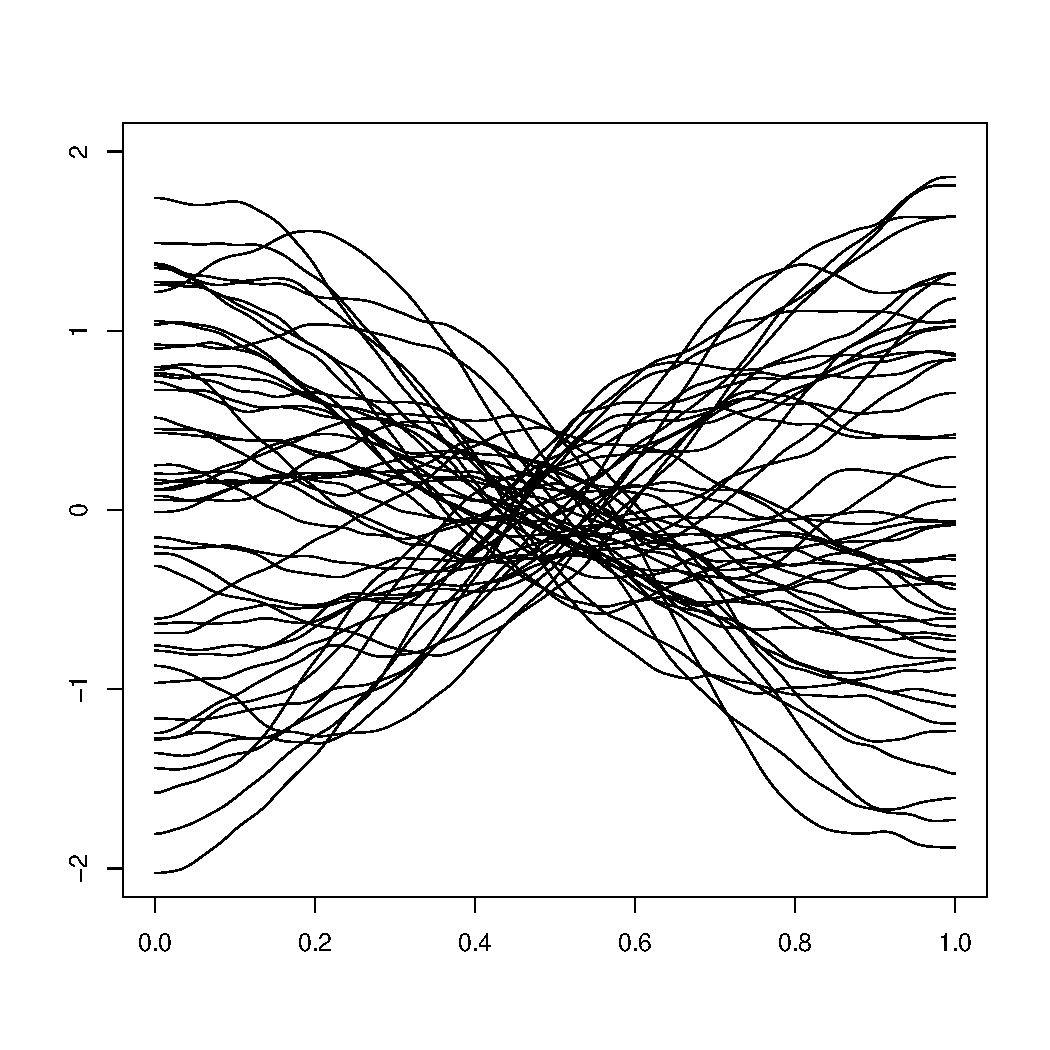
\includegraphics[width=\textwidth]{Plots/Images-nonparametric/cy-curves.pdf}
                \caption{}
                \label{}
        \end{subfigure}
         \begin{subfigure}[b]{0.34\textwidth}
                \centering
                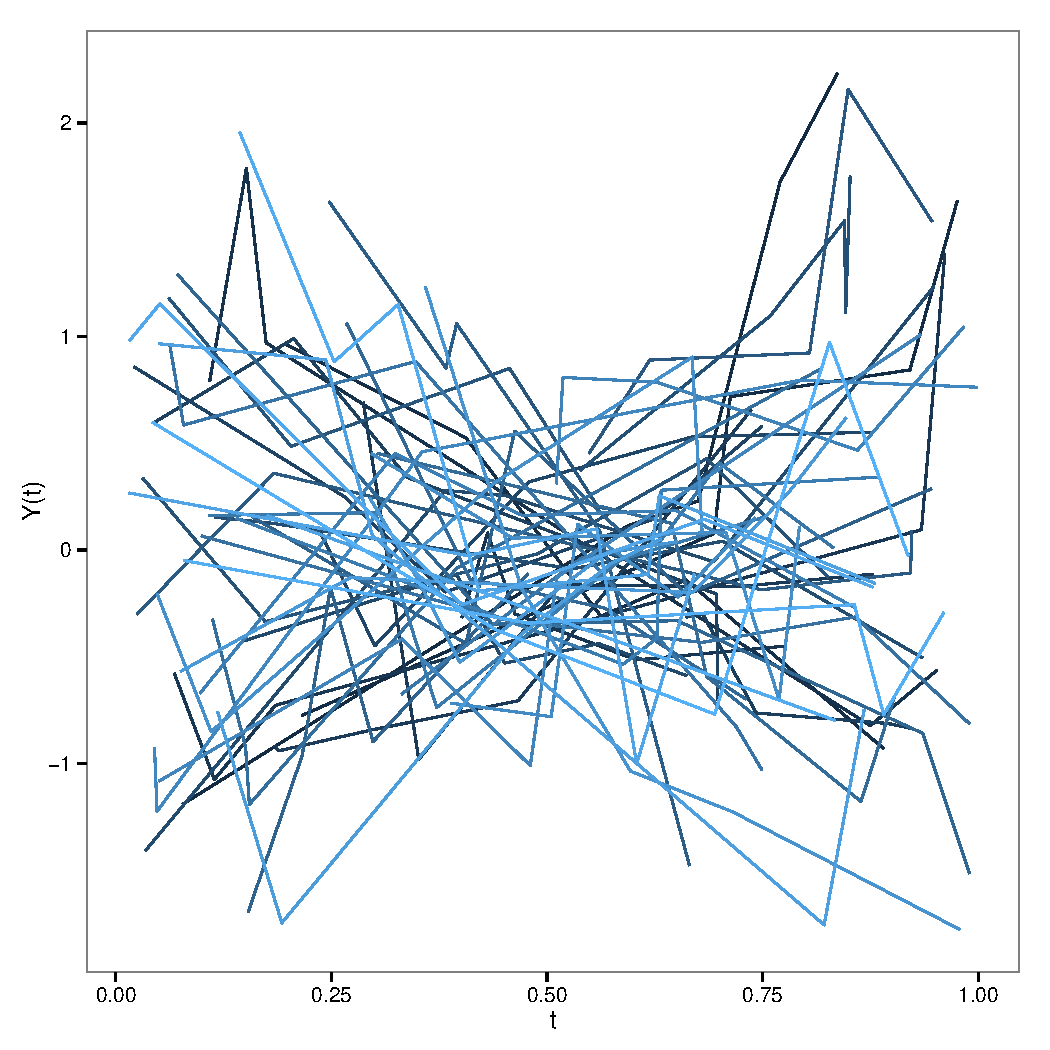
\includegraphics[width=\textwidth]{Plots/Images-nonparametric/cy-data-m5.pdf}
                \caption{}
                \label{}
        \end{subfigure}

        \begin{subfigure}[b]{0.34\textwidth}
                \centering
                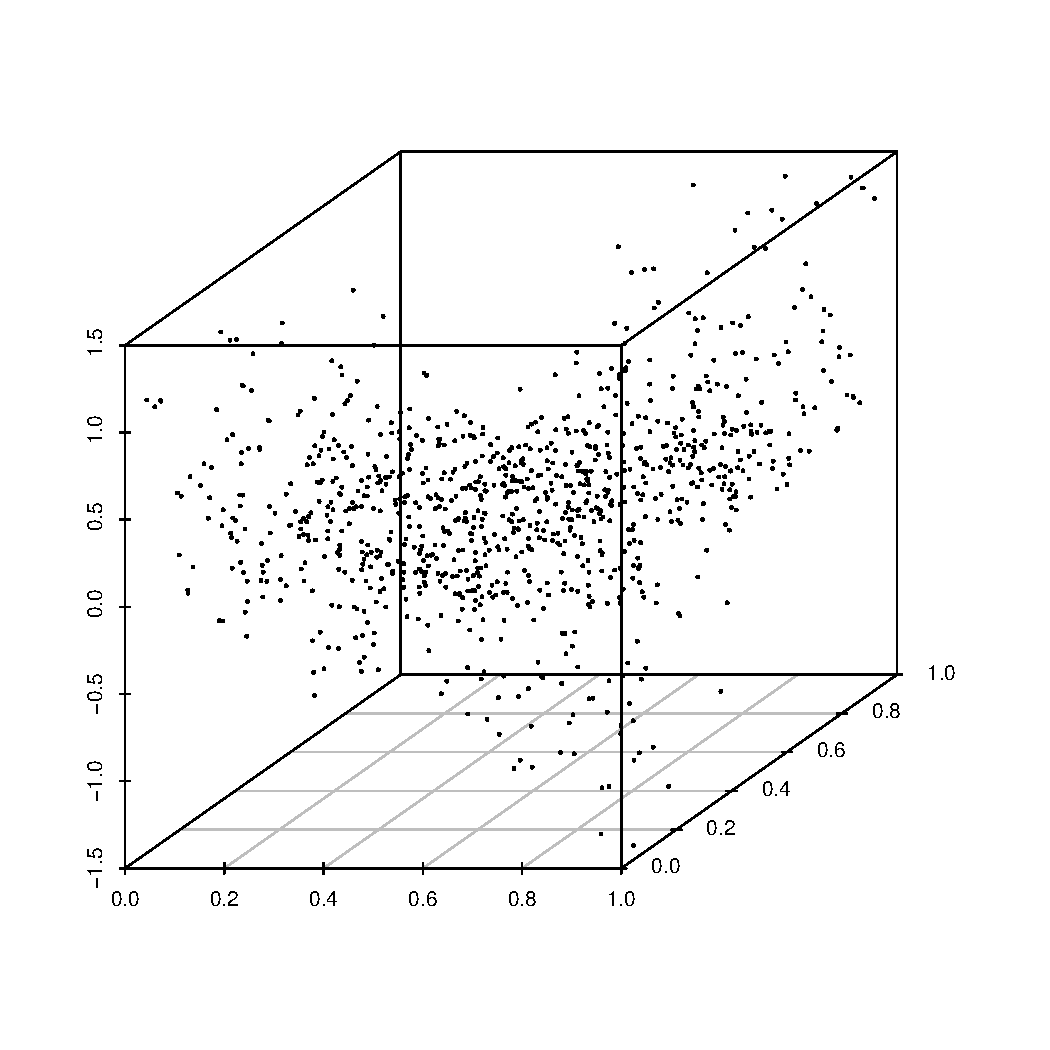
\includegraphics[width=\textwidth]{Plots/Images-nonparametric/cy-scatter3d-m5.pdf}
                \caption{}
                \label{}
        \end{subfigure}%
          \begin{subfigure}[b]{0.34\textwidth}
                \centering
                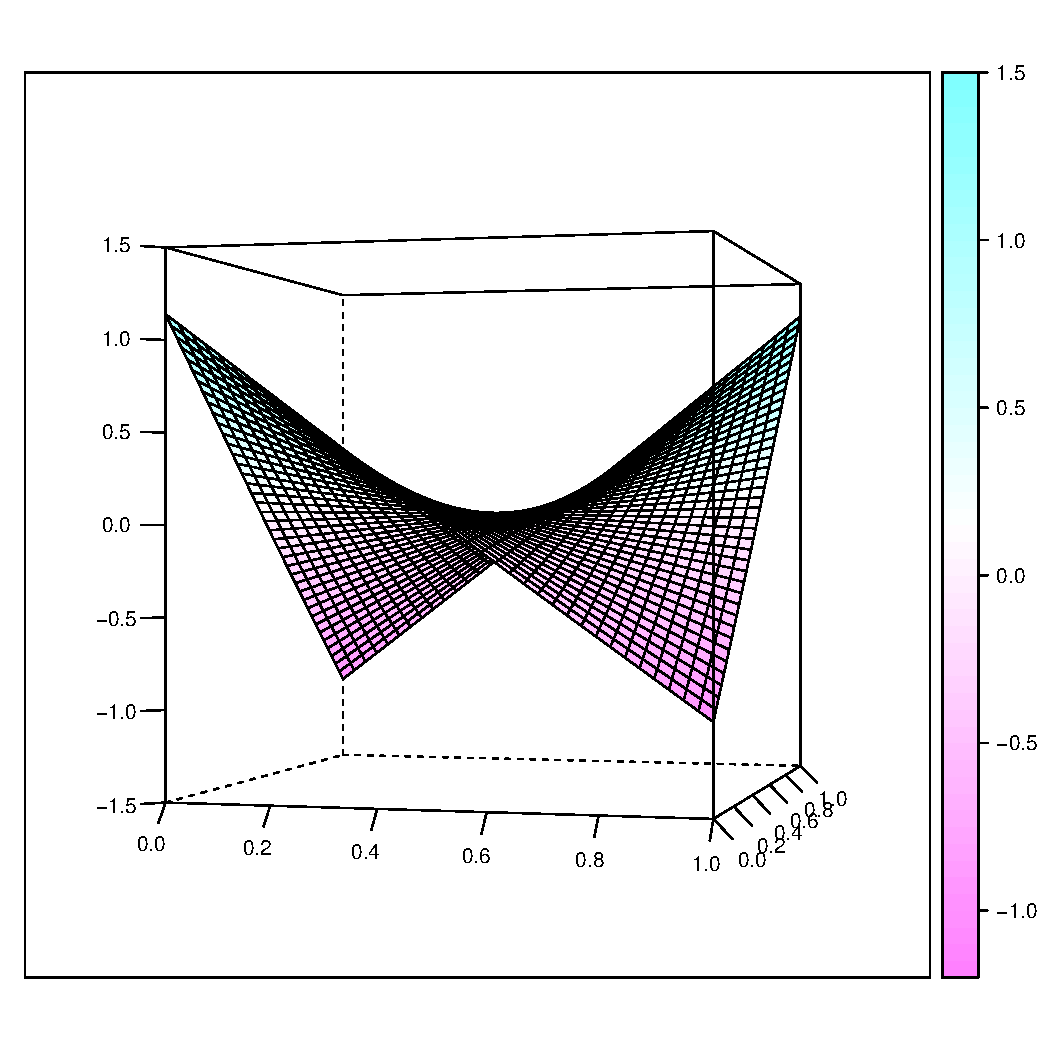
\includegraphics[width=\textwidth]{Plots/Images-nonparametric/cy-fit-wireframe-m5.pdf}
                \caption{}
                \label{}
        \end{subfigure}%
%        \caption{(a) 50 simulated curves from the process $X(t)$ in \eqref{eq:sim process} (b) data set of curves evaluated at five random locations with noise, $\sigma_0=0.392$ (c) Scatterplot of values based on the data used to estimate covariance surface (d) Estimated covariance function. }
%        \label{fig:sim curves}
 \end{figure}
}

\frame{
\begin{figure}
 	\centering   
        \begin{subfigure}[b]{.30\textwidth}
                \centering
                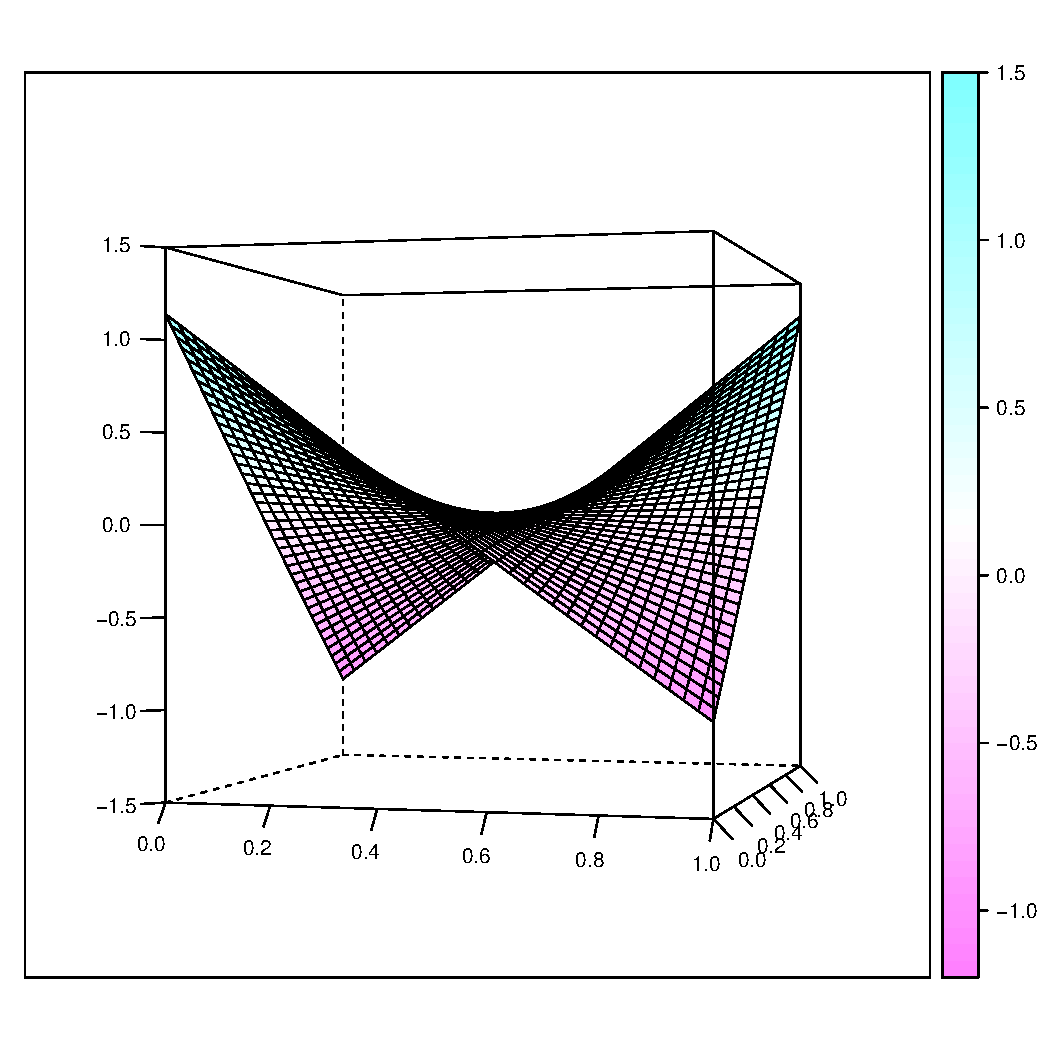
\includegraphics[width=\textwidth]{Plots/Images-nonparametric/cy-fit-wireframe-m5.pdf}
                \caption{m = 5}
                \label{}
        \end{subfigure}%
        \begin{subfigure}[b]{.30\textwidth}
                \centering
                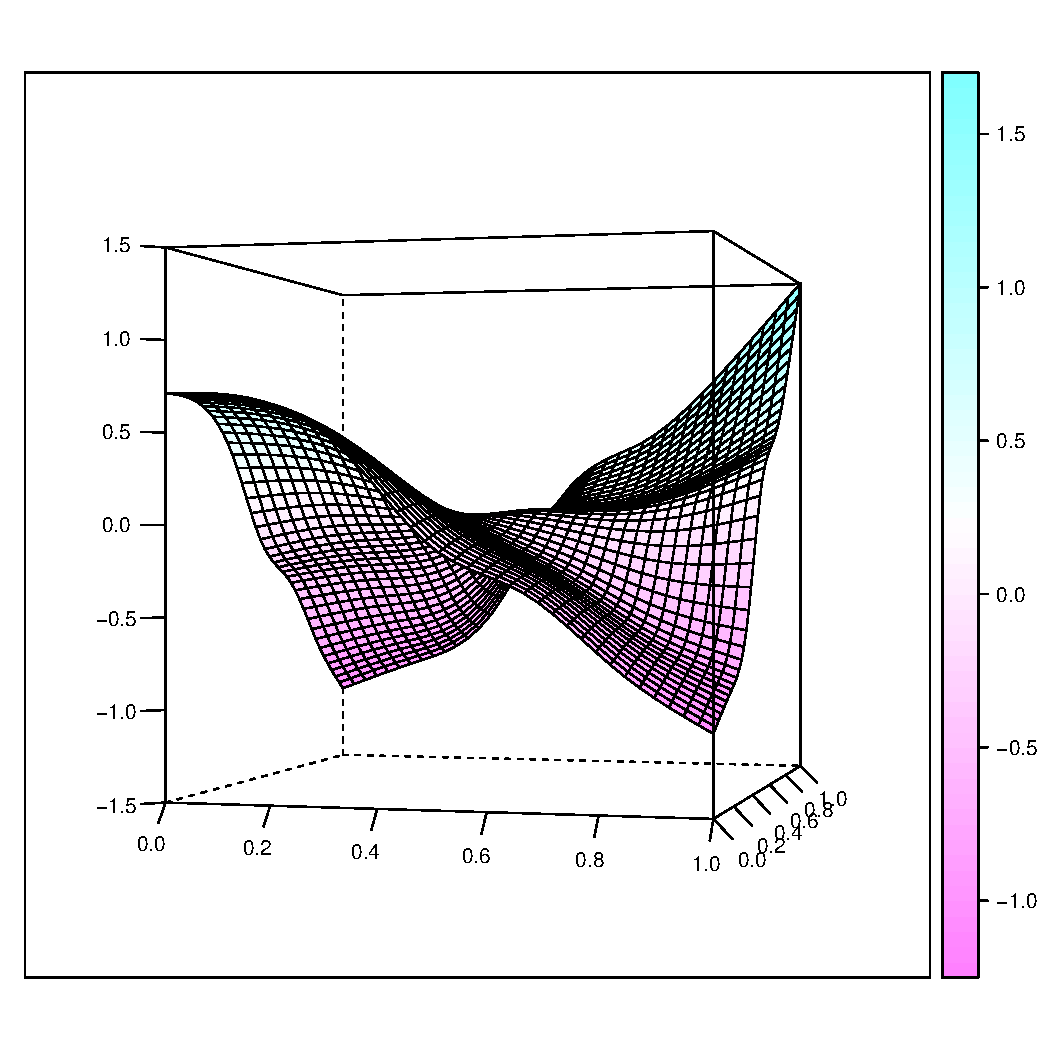
\includegraphics[width=\textwidth]{Plots/Images-nonparametric/cy-fit-wireframe-m10.pdf}
                \caption{m = 10}
                \label{}
        \end{subfigure}

        \begin{subfigure}[b]{.30\textwidth}
                \centering
                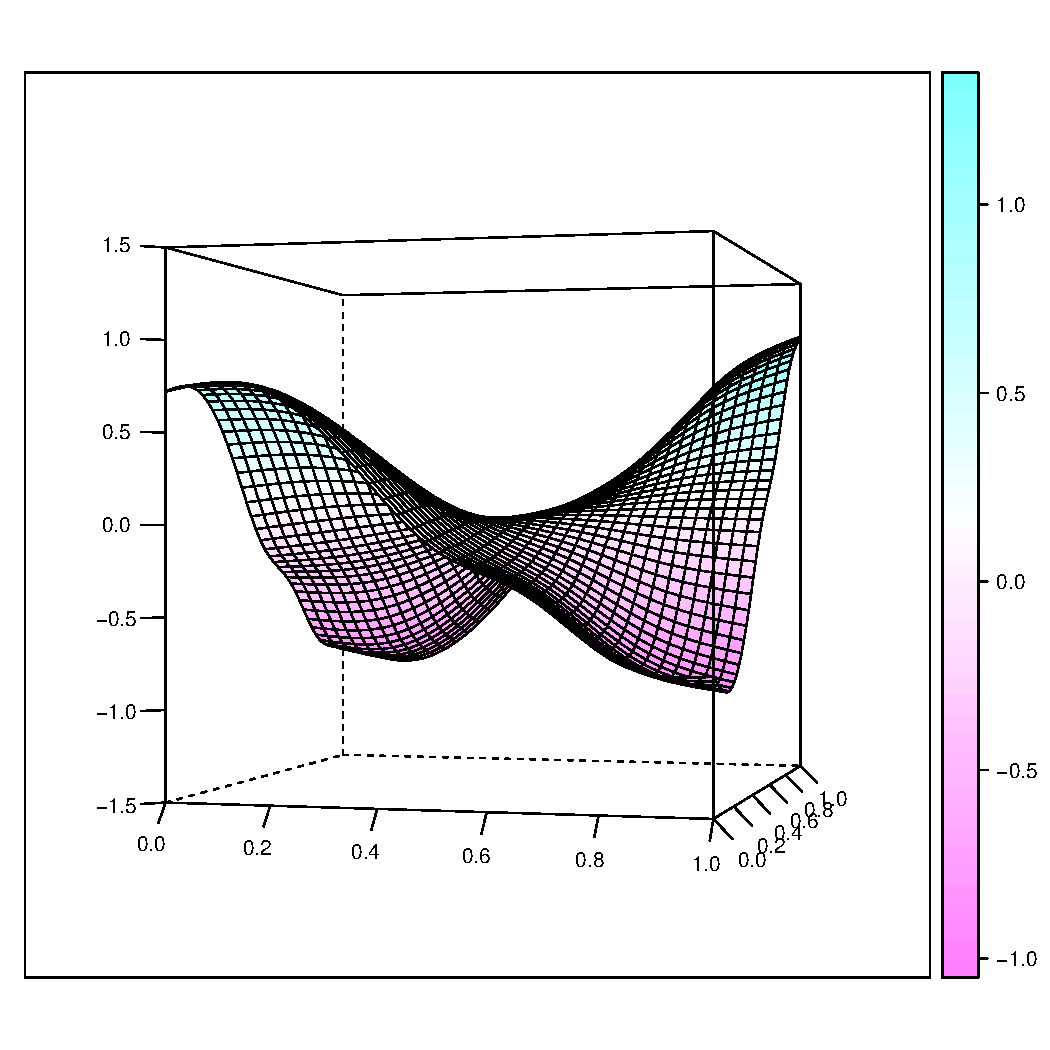
\includegraphics[width=\textwidth]{Plots/Images-nonparametric/cy-fit-wireframe-m40.pdf}
                \caption{m = 40}
                \label{}
        \end{subfigure}
                \begin{subfigure}[b]{.30\textwidth}
                \centering
                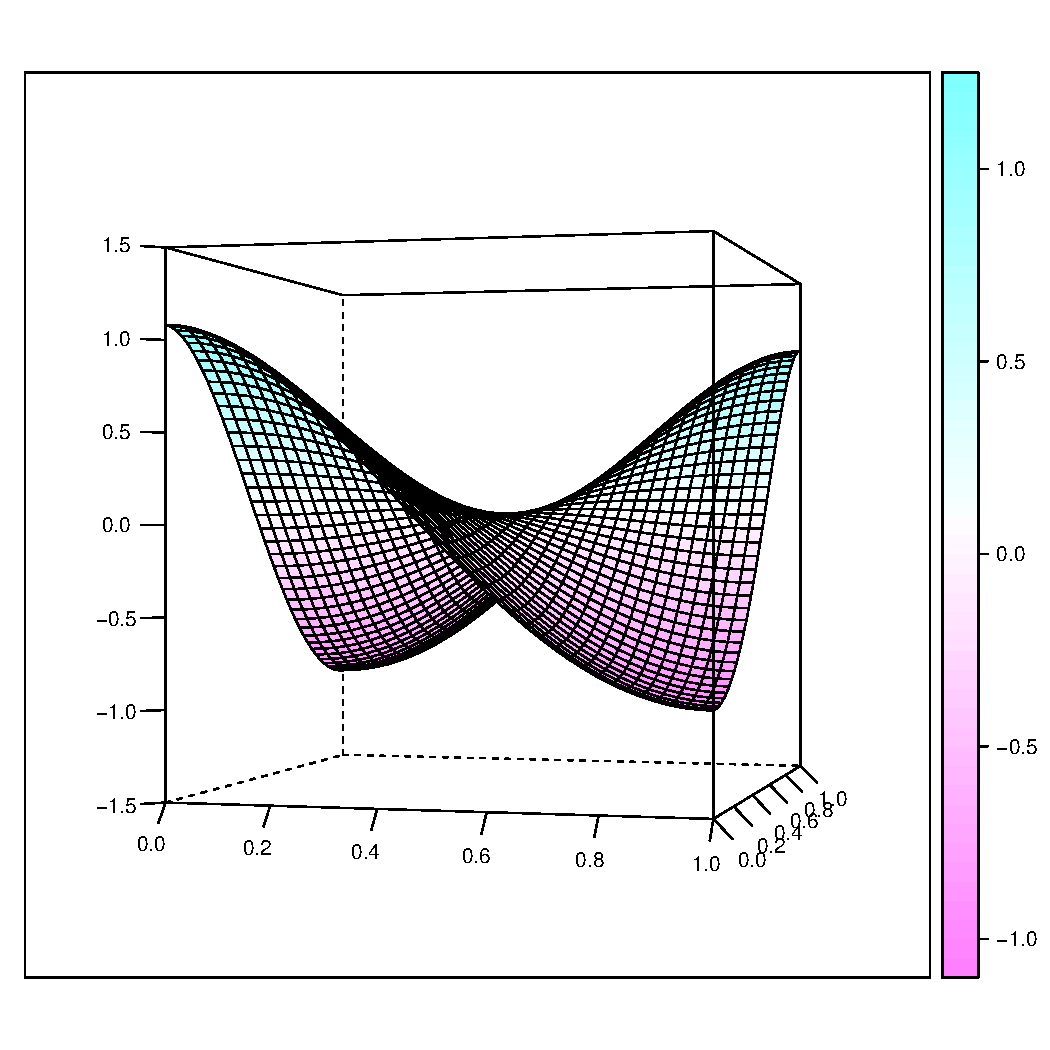
\includegraphics[width=\textwidth]{Plots/Images-nonparametric/cy-true-wireframe.pdf}
                \caption{truth}
                \label{}
        \end{subfigure}
\end{figure}
}


\begin{frame}
\frametitle{Functional Principal Components}
To the covariance $C(s,t)$ has the following representation 
\begin{equation*} 
 C(s,t) = \sum_{i=1}^{\infty}\lambda_i\psi_i(s)\psi_i(t),
\end{equation*}
\begin{itemize}
\item  $\{\psi_m(t)\}_{m=1,2,\ldots}$ are orthonormal (in $L_2$) eigenfunctions
\item  $\{\lambda_m \}_{m=1,2,\ldots}$ are nonnegative and nondecreasing eigenvalues. 
\item eigenfunctions satisfy $\int_a^bC(s,t)\psi_j(t)dt = \lambda_j\psi_j(t)$. 
\end{itemize}
Karhunen-Loeve theorem $\rightarrow$ $X(t)$ admits the representation
\begin{equation*}
X(t) =  \sum_{m=1}^{\infty}\alpha_m \psi_m(t), \mbox{ where  } \alpha_m = \int_a^b X(t) \psi_m(t)dt,
\end{equation*}
\begin{itemize}
\item $\{\alpha_m \}_{m=1,2,\ldots}$ are uncorrelated random variables
\item $E(\alpha_m)=0$ and Var($\alpha_m$) = $\lambda_m$, $\sum_m \lambda_m < \infty$. 
\end{itemize}
\end{frame}

\frame{

We seek functions $\hat{\psi}(s)$ that satisfy
\begin{equation*} \label{eq:eigenfuns}
\int \hat{C}(s,t)\hat{\psi}(t)dt=\theta\hat{\psi}(s).
\end{equation*}
\begin{itemize}
\item Idea: adapt methods developed for finite basis representations.
\item Let
\begin{equation}
\mathbf{g(\cdot)}=(1, k_1(\cdot),R_{1}(\cdot, t_1),R_{1}(\cdot, t_2),\dots, R_{1}(\cdot, t_K))'.
\label{eq:g}
\end{equation}
\item Need to represent $\hat{C}(s,t)= \mathbf{g}(s)'A\mathbf{g}(t)$ for some matrix $A$. See next slide...
\end{itemize}
}

\begin{frame}[shrink=10]
Using $\mathbf{g}$ in \eqref{eq:g} the covariance function estimator has the representation $\hat{C}(s,t)= \mathbf{g}(s)'A\mathbf{g}(t)$ where
\vspace{0.8cm}
\begin{center}
 $A = \left(\begin{array}{cc:cccc}
d_{00,00} & d_{01,00} & c_{1.} & c_{2.} & \dots & c_{K.}\\
d_{00,01} & d_{01,01} & \sum_j c_{1j}k_1(t_j) & \sum_j c_{2j}k_1(t_j) & \dots & \sum_j c_{Kj}k_1(t_j)\\
\hdashline
c_{.1}   & \sum_j c_{j1}k_1(t_j) & c_{11}   & c_{12}   & \dots & c_{1K}\\
c_{.2}   & \sum_j c_{j2}k_1(t_j) & c_{21}   & c_{22}   & \dots & c_{2K}\\
\vdots  & \vdots                            & \vdots    & \vdots & \ddots    & \vdots \\
c_{.K}   & \sum_j c_{jK}k_1(t_j) & c_{K1}   & c_{K2}   & \dots & c_{KK}
\end{array}\right)$
\end{center}
\end{frame}

\frame{
The following result states that the eigenfunctions can be expressed as a linear combination of the elements of $\mathbf{g}$.
\begin{lemma} \label{thm:eigenfunctions}
	The eigenfunctions of $\hat{C}(s,t)$ can be expressed as
	\begin{equation*}
		\hat{\psi}_k(\cdot) = b'_k\mathbf{g}(\cdot),	
	\end{equation*}
	where $Q$ is defined to be
\begin{equation*}
	Q_{ij} = \int_0^1\mathbf{g_i}(t)\mathbf{g}_j(t)dt,
\end{equation*}
	$b_k$ is the $k$-th column of $B=Q^{-1/2}U$ and $U$ is the eigenvectors of $Q^{1/2}AQ^{1/2}$, and 
\[
\mathbf{g(\cdot)}=(1, k_1(\cdot),R_{1}(\cdot, t_1),R_{1}(\cdot, t_2),\dots, R_{1}(\cdot, t_K))'.
\]
\end{lemma}
}


\frame{
\frametitle{Discussion}
\begin{itemize}
\item  Allows smoothing penalty to be more directly connected to the curves (i.e. the scientific process being observed). 
\item Simulation indicate the estimator performs well even with sparsely observed curves. 
\item Method is general and could easily be applied to a penalty based on arbitrary linear differential operators. 
\item We have also created an R package implementation, making it convenient to use empirical basis representation for functional data analyses. 
\end{itemize}
}


%%%%% PHENOLOGY %%%%%
\frame{
\begin{center}
FUNCTIONAL DATA ANALYSIS OF SATELLITE MEASUREMENTS OF PHENOLOGICAL PROCESSES
\end{center}
}
\begin{frame}
\frametitle{Introduction}
\begin{itemize}
\item \emph{Phenology} is the study of annual life-cycles of terrestrial vegetation and how they are effected by climate change or other environmental variables (e.g. elevation). 

\item Understanding vegetation phenology and its spatio-temporal variation is required to reveal and predict ongoing changes in Earth system dynamics. \\[0.5cm]

\item \textbf{Goal}: Develop a flexible model for vegetation life-cycles.  A single life-cycle is determined by two variables: 
\begin{itemize} 
\item Onset of Greenness (OG) and 
\item End of Senescence (ES).
\end{itemize}
\end{itemize}
\end{frame}

\frame
{
\frametitle{Defining Vegetation Life-cycles}
\begin{figure}
   \begin{center}
   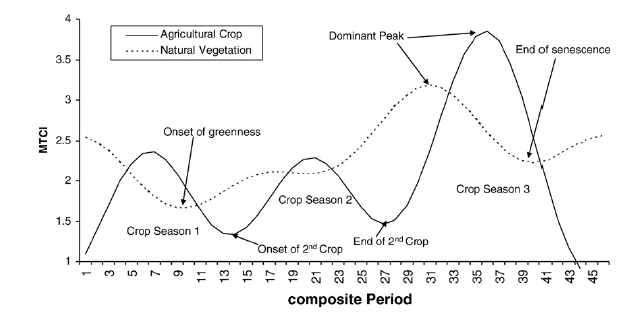
\includegraphics[width=1.1\linewidth]{Plots/PhenoVars_Jegan.png} 
   %\caption{Diagram illustrating typical phenology patterns for agricultural land and natural vegetation. }
\end{center}
\end{figure}
}

\frame
{
\frametitle{Data processing and analysis flow chart }
\begin{figure} %  figure placement: here, top, bottom, or page
   \begin{center}
   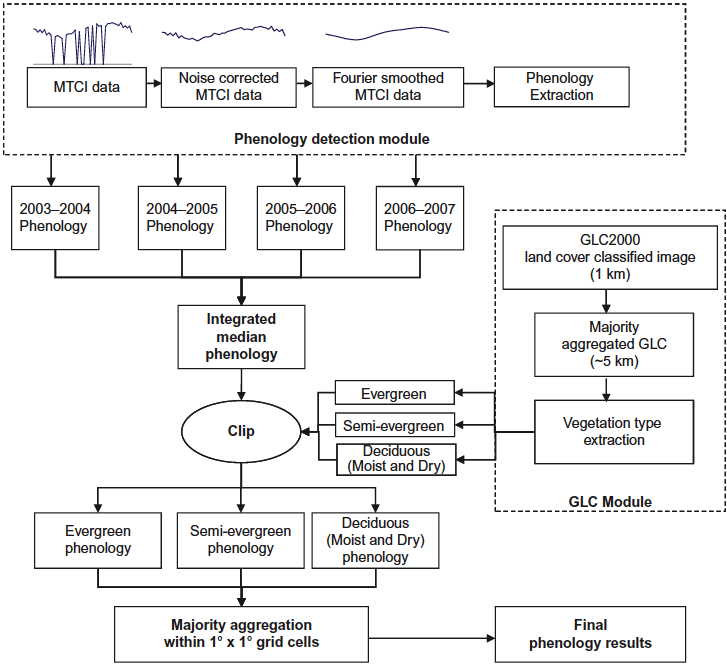
\includegraphics[width=0.7\linewidth]{Plots/PhenoScheme.png} 
%   \caption{example caption}
   %\label{fig:example}
   \end{center}
\end{figure}
}

\frame
{
\frametitle{Data processing and analysis flow chart }
\begin{figure} %  figure placement: here, top, bottom, or page
   \begin{center}
   \includegraphics[width=\linewidth]{Plots/pheno-diagram.png} 
%   \caption{example caption}
   %\label{fig:example}
   \end{center}
\end{figure}
}




